%%%%%%%%%%%%%%%%%%%%%%%%%%%%% Infrared Data Reduction Techniques %%%%%%%%%%%%%%%%%%%%

\chapter{Infrared Astronomy and Data Reduction Techniques}
\label{cha:InfraredDataReductionTechniques}

In this chapter, we introduce both photometry and spectroscopy and explore the data reduction techniques we employed to process our observations of a target system. %

%%%%%%%%%%%%%%%%%%%%%%%%%%%%% The Magnitude Scale %%%%%%%%%%%%%%%%%%%%

\section{Photometry and the Magnitude Scale}
\label{cha:InfraredDataReductionTechniques:sec:MagnitudeScale}

Part of this thesis is concerned with determining and modelling the
variation in brightness of our observations of our target system. The brightness of this system is measured by a technique known as \textbf{photometry}, %
and the brightness of the object is measured in \textbf{magnitudes}, %
an astronomical scale based on increasing
brightness with decreasing magnitude. %
(This scale dates back to the Greek astronomer Hipparchus in
the second century B.C.) %

\vspace{\myparskip}

We normally measure the luminosity of the binary over a
small range of wavelengths, known as a%
\ \textbf{photometric band}, rather than measuring the brightness over the entire
electromagnetic spectrum. The bands we selected for the observations in this thesis were the $J$--
(1.06--1.44$\,\mu \mathrm{m}$), $K$-- (1.96--2.44$\,\mu \mathrm{m}$) and
$K_s$-- (1.99--2.31$\,\mu\mathrm{m}$)%
\footnote{%
\label{cha:InfraredDataReductionTechniques:sec:MagnitudeScale:subsec:Photometry:foot:Ks}
The $K_s$ (``$K$ short'') filter is a modified K filter
that reduces the thermal background for warm ground-based
telescopes, as the background at these wavelengths can be significant.}%
\ bands. %

\vspace{\myparskip}

The magnitude of the binary measured by the detector is known as the \textbf{instrumental magnitude}.%
\ Since this value will vary depending on various factors, such as the photometric conditions and the airmass of the observation, this value can not be immediately compared with earlier observations. We must first make the following corrections, in order to make such comparisons. %

%%%%%%%%%%%%%%%%%%%%%%%%%%%%% Atmospheric Extinction %%%%%%%%%%%%%%%%%%%%

\subsection{Atmospheric Extinction}
\label{cha:InfraredDataReductionTechniques:sec:MagnitudeScale:subsec:AtmosphericExtinction}

When a star is observed through the atmosphere, the star is obscured
due to the absorption and scattering of the starlight by the
atmosphere, a phenomenon known as \textbf{atmospheric extinction}. %

\vspace{\myparskip}

The amount of extinction for a certain wavelength is known as the \textbf{(atmospheric) extinction} %
for that wavelength, and is given by the product of the
\textbf{airmass ($\Chi$)} %
\label{cha:InfraredDataReductionTechniques:sec:MagnitudeScale:subsec:AtmosphericExtinction:topic:k}
and the \textbf{extinction coefficient ($k$)}.%
\ The airmass is approximately the inverse cosine of the zenith angle of
the telescope, and the extinction coefficient is the number of
magnitudes of extinction per unit airmass. The value of this coefficient depends on
the wavelength observed and the location of the observatory. %

\vspace{\myparskip}

If we determine this atmospheric extinction, we can then combine our corrected measurement with that of a photometric standard of known magnitude to obtain the \textbf{apparent
magnitude} %
of our target star. This magnitude can be compared to other observations, assuming similar photometric conditions. %

%%%%%%%%%%%%%%%%%%%%%%%%%%%%% Interstellar Extinction %%%%%%%%%%%%%%%%%%%%

\subsection{Interstellar Extinction}
\label{cha:InfraredDataReductionTechniques:sec:MagnitudeScale:subsec:InterstellarExtinction}

We must also consider the absorption and scattering of starlight due to the
dense dust clouds which lie between the Earth and the star. This is
known as \textbf{interstellar extinction}. %

\vspace{\myparskip}

The number of magnitudes of obscuration at a certain wavelength
$\lambda$ is known as the \textbf{(interstellar) extinction $A_{\lambda}$}. %
We can then define two quantities: the \textbf{reddening
($E_{B-V}$)} is the difference $A_B - A_V$, where $B$ is the blue
(390--490 nm) passband and $V$ is the visible (500--600 nm) passband,
and the \textbf{extinction ratio, $R_V$}, which is the ratio of the visible extinction to the reddening.
This ratio varies, but is usually approximated as
\begin{eqnarray}
\label{cha:InfraredDataReductionTechniques:sec:MagnitudeScale:subsec:InterstellarExtinction:eqn:rv}
R_V = \frac{A_V}{E_{B-V}} \sim 3.1.
\end{eqnarray}
(See, for example, %
\citeNP{CardelliClaytonMathis:1989}.)%

\vspace{\myparskip}

To correct for interstellar extinction at a given wavelength, we can use the results of \citeN{CardelliClaytonMathis:1989}, who derived the following values for the ratios between the interstellar
extinction in the $K$--band ($A_K$) and the $J$--band ($A_J$), and that
in the $V$--band ($A_V$):
\begin{eqnarray}
\label{cha:InfraredDataReductionTechniques:sec:MagnitudeScale:subsec:InterstellarExtinction:eqn:CardelliA}
\frac{A_K}{A_V} = 0.114,\\\nonumber
\frac{A_J}{A_V} = 0.282.
\end{eqnarray}
We can therefore determine an expression for, say, $A_K$, as follows:
\begin{eqnarray}
\label{cha:InfraredDataReductionTechniques:sec:MagnitudeScale:subsec:InterstellarExtinctioneqn:CardelliAK}
A_K & = & 0.114 \times A_V, \\\nonumber
    & = & 0.114 \times R_V \times E_{B-V},
\end{eqnarray}
and then insert the value for $R_{V}$ (see Equation~\ref{cha:InfraredDataReductionTechniques:sec:MagnitudeScale:subsec:InterstellarExtinction:eqn:rv}) and our measured value for $E_{B-V}$.%

\vspace{\myparskip}

We can then correct the apparent magnitude of the star for the
obscuration due to the interstellar medium to obtain the \textbf{dereddened
magnitude} of the star.

%%%%%%%%%%%%%%%%%%%%%%%%%%%%% Absolute Magnitude %%%%%%%%%%%%%%%%%%%%

\subsection{The Intrinsic Brightness of a Star}
\label{cha:InfraredDataReductionTechniques:sec:MagnitudeScale:subsec:AbsoluteMagnitude}

The final correction that may be made to the magnitude of a star is to
account for the distance to the star. For example, although the $V$--band magnitude of our Sun is $-26.8$, at a distance of 10 parsecs it would
appear as a star of magnitude 4.72. In order to be able to catalog a star according
to its intrinsic brightness, we calculate its \textbf{absolute
magnitude ($M$)}. This is defined as the magnitude of the star if observed at a distance
of 10 parsecs (pc), and is given by:
\begin{eqnarray}
\label{cha:InfraredDataReductionTechniques:sec:MagnitudeScale:subsec:AbsoluteMagnitude:eqn:AbsMag}
M & = & m - 5 \log{\frac{d}{10\,pc}},
\end{eqnarray}
where $m$ is the dereddened magnitude of the star, and $d$ is its
distance. For example, the absolute $K$--band magnitude is given by:
\begin{eqnarray}
\label{cha:InfraredDataReductionTechniques:sec:MagnitudeScale:subsec:AbsoluteMagnitude:eqn:AbsMagK}
M_K & = & K_0 - 5 \log{\frac{d}{10\,pc}},
\end{eqnarray}
where $K_0$ is the dereddened $K$--band magnitude of the star. A
similar equation holds for the $J$--band:
\begin{eqnarray}
\label{cha:InfraredDataReductionTechniques:sec:MagnitudeScale:subsec:AbsoluteMagnitude:eqn:AbsMagJ}
M_J & = & J_0 - 5 \log{\frac{d}{10\,pc}}.
\end{eqnarray}

%%%%%%%%%%%%%%%%%%%%%%%%%%%%% Spectroscopy %%%%%%%%%%%%%%%%%%%

\section{Spectroscopy}
\label{cha:InfraredDataReductionTechniques:sec:Spectroscopy}

As well as measuring the amount of light from a celestial object using
photometry, we can also study the spectrum of that light. This is
known as \textbf{spectroscopy}. The first application of spectroscopy was the identification of Sodium
in the solar spectrum by Fraunhofer in 1814, and the element Helium was discovered spectroscopically in 1868 by studying the Sun. Since
these observations, spectroscopy has been employed to determine the
chemical makeup of the Sun and other stars. %

\vspace{\myparskip}

In this thesis, we need to determine whether there are emission or absorption features present in the spectrum of a binary system, and how strong the spectral features are relative to those in a comparison star. We measure the strength of a spectral
feature by calculating the \textbf{equivalent width} of the line. %

%%%%%%%%%%%%%%%%%%%%%%%%%%%%% Equivalent Width %%%%%%%%%%%%%%%%%%%%

\subsection{The Equivalent Width of a Spectral Feature}
\label{cha:InfraredDataReductionTechniques:sec:Spectroscopy:subsec:EquivalentWidth}

The \textbf{equivalent width} of a spectral absorption or emission line is a measure of the strength
of the feature, and is defined as the width of a perfectly black line
having the same total absorption or emission as the real line. It can
be expressed as:
\begin{eqnarray}
\label{cha:InfraredDataReductionTechniques:sec:Spectroscopy:subsec:EquivalentWidth:eqn:equiv}
|W| = \int \frac{F_c - F_{\lambda}}{F_c} d\lambda,
\end{eqnarray}
where $F_c$ is the flux due to the continuum, $F_{\lambda}$ is the
flux at wavelength $\lambda$, and the integral is taken from one side
of the spectral line to the other. Absorption features are denoted by
positive equivalent widths, and emission features by negative
widths. Equivalent widths are usually given in Angstroms (\AA). %

\vspace{\myparskip}

The equivalent width of a spectral line can be thought of as the width
of a box of the same area as is under the line, and whose height is the
continuum flux value. An example of such a representation is given in
Figure~%
\vref{cha:InfraredDataReductionTechniques:sec:Spectroscopy:subsec:EquivalentWidth:fig:CarrollEquiv}%
. %

%%%%%%%%%%%%%%%%%%%%%%%%%%%%% CarrollEquiv %%%%%%%%%%%%%%%%%%%%
\begin{figure}[!htb]
\begin{center}
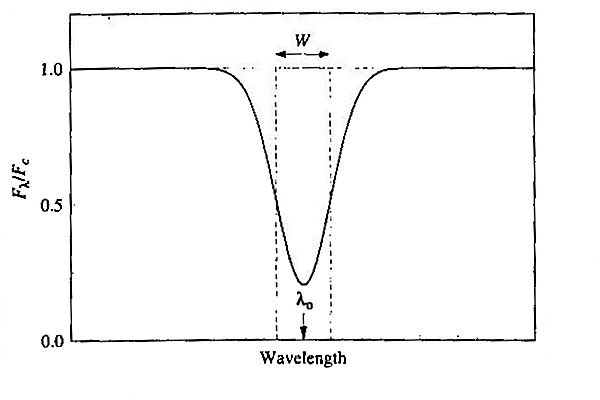
\includegraphics[width=5.0in]{CarrollEquiv}
\caption{%
Example of a spectral absorption line at $\lambda=\lambda_0$,
indicating the equivalent width $W$ of the
feature (Carroll \& Ostlie 1996). }%
\label{cha:InfraredDataReductionTechniques:sec:Spectroscopy:subsec:EquivalentWidth:fig:CarrollEquiv}
\end{center}
\end{figure}
%%%%%%%%%%%%%%%%%%%%%%%%%%%%%%%%%%%%%%%%%%%%%%%%%%%%%%%%%%%%%%%%%%

\nocite{CarrollOstlie:1996}

%%%%%%%%%%%%%%%%%%%%%%%%%%%%% Radial Velocity %%%%%%%%%%%%%%%%%%%%

\subsection{The Radial Velocity of the Secondary Star}
\label{cha:InfraredDataReductionTechniques:sec:Spectroscopy:subsec:RadialVelocity}

We used spectroscopy in order to verify that the disk in our target system was not contaminating the light curve of the binary. We also measured the \textbf{radial velocity} of the secondary star, so as to confirm that our spectra were consistent with past observations. This was especially necessary as these were the first high signal-to-noise $K$--band spectra of a black hole X--ray
transient system.

\vspace{\myparskip}

The radial velocity of the secondary star in a
binary system may be calculated from:
\begin{eqnarray}
\label{cha:InfraredDataReductionTechniques:sec:Spectroscopy:subsec:RadialVelocity:eqn:Vr}
v_r = \gamma + K_2 \sin{(2\pi\phi)},
\end{eqnarray}
where $\gamma$ is the systematic velocity of the binary system, and
$\phi$ is the orbital phase of the binary.

\vspace{\myparskip}

The radial velocity can be measured from the
Doppler shift of the observed wavelengths of the spectral features
in the spectrum of the star, which is a result of the motion of the star relative to the observer along their line of sight. This shift is given by:%
\begin{eqnarray}
\label{cha:InfraredDataReductionTechniques:sec:Spectroscopy:subsec:RadialVelocity:eqn:shift}
\Delta\lambda     & = & \lambda_{\mathrm{obs}} - \lambda,\\
               & = & \frac{v_r \lambda}{c},
\end{eqnarray}
where $\lambda$ and $\lambda_{\mathrm{obs}}$ are the rest and
observed wavelengths, respectively, of the spectral
feature. Therefore, if we know $\Delta\lambda$, we can also calculate the
radial velocity from:%
\begin{eqnarray}
\label{cha:InfraredDataReductionTechniques:sec:Spectroscopy:subsec:RadialVelocity:eqn:vr2}
v_r = \frac{\Delta\lambda}{\lambda} c.
\end{eqnarray}

\vspace{\myparskip}

We compared the predicted radial velocity of our target star
(calculated using the published spectroscopic ephemeris) with that
determined from the $\Delta\lambda$ measured from the spectrum of the star, to ensure that our result agreed with prior observations of \groj. %

%%%%%%%%%%%%%%%%%%%%%%%%%%%%% Infrared Astronomy %%%%%%%%%%%%%%%%%%%%

\section{Advantages of IR Observations of \groj}
\label{cha:InfraredDataReductionTechniques:sec:InfraredAstronomy}

This thesis is concerned with the infrared observations of the X--ray binary\\%
% WHITE SPACE %
\groj. Although X--ray binaries emit energy primarily as X--rays, our
observations of \groj\ were made at infrared wavelengths,
(the $J$--, $K$-- and $K_{s}$--bands). This section explains the
advantages for doing so, as well as the drawbacks of infrared
observations. %

%%%%%%%%%%%%%%%%%%%%%%%%%%%%% Dominance of Secondary %%%%%%%%%%%%%%%%%%%%

\subsubsection{Dominance of Secondary}
\label{cha:InfraredDataReductionTechniques:sec:InfraredAstronomy:subsubsec:DominanceOfSecondary}


A luminous accretion disk in a binary system will be bluer than the secondary star, and should contribute less in the infrared than in the optical. Hence this intrinsic emission from the secondary star should dominate in the infrared, and this will allow a better estimate of the brightness of the secondary to be made. This increases the likelihood of tightly constraining the mass ratio, inclination and black hole mass through infrared observations. %

%%%%%%%%%%%%%%%%%%%%%%%%%%%%% Infrared Spectroscopy %%%%%%%%%%%%%%%%%%%%

\subsubsection{Disk Contamination and Infrared Spectroscopy}
\label{cha:InfraredDataReductionTechniques:sec:InfraredAstronomy:subsubsec:InfraredSpectroscopy}

If we ignore the accretion disk contribution for a given binary
system, we cannot be certain that we are not underestimating the
orbital inclination for that system, or that our derived stellar masses are valid estimates. %
Although the quiescent infrared disk contribution is often
assumed be negligible (see, for example, %
\citeNP{ShahbazNaylorCharles:1994}%
), it is possible that the disk can in fact be a
strong source of infrared radiation.
Infrared spectroscopy can be used to constrain the level of
accretion disk contamination in the infrared during
quiescence. %

%%%%%%%%%%%%%%%%%%%%%%%%%%%%% Interstellar Extinction %%%%%%%%%%%%%%%%%%%%

\subsubsection{Interstellar Extinction}
\label{cha:InfraredDataReductionTechniques:sec:InfraredAstronomy:subsubsec:InterstellarExtinction}

In general, the $K$--band interstellar extinction, $A_K$, is nine times smaller
 than visual band extinction, $A_V$ ($A_K \sim 0.114\ A_V$: %
\citeNP{CardelliClaytonMathis:1989}). Therefore, the interstellar medium absorbs less infrared radiation
than optical. Hence any attempt to locate a faint distant object may be more
successful if the observations are made in the infrared. %

\vspace{\myparskip}

More specifically, we will later show that our target system \groj\ has a high visual extinction of $A_{V} =4.0\pm0.3$\,mag, but a low infrared extinction $A_{K} = 0.42\pm0.04$\,mag (see \S~\vref{cha:lightcurve:sec:Photometry:subsec:DereddenedMagnitude}). This system is therefore
less obscured in the infrared, which improves the quality of images taken at these wavelengths. %

%%%%%%%%%%%%%%%%%%%%%%%%%%%%% Improved Resolution %%%%%%%%%%%%%%%%%%%%

\subsubsection{Improved Spatial Resolution}
\label{cha:InfraredDataReductionTechniques:sec:InfraredAstronomy:subsubsec:ImprovedResolution}

More generally, the resolution of an observation specifies the minimum angular
separation required between two stars for the pair to be
distinguishable. At wavelengths less than or equal to infrared wavelengths
(1.0--2.4$\,\mu \mathrm{m}$), and for 1-m or larger telescopes, this
resolution is determined mainly by the effect of turbulence in the
atmosphere (see, e.g., %
\citeNP{Schroeder:1987:Resolution}%
\ for details). In this regime, there is an improvement in resolution
with increasing wavelength, as the longer wavelengths are less
refracted by the atmosphere than the shorter wavelengths. Therefore,
the infrared offers better quality images than the optical
(400--700\,nm). %

%%%%%%%%%%%%%%%%%%%%%%%%%%%%% Disadvantages %%%%%%%%%%%%%%%%%%%%

\subsubsection{Disadvantages}
\label{cha:InfraredDataReductionTechniques:sec:InfraredAstronomy:subsubsec:Disadvantages}

The main disadvantage of infrared photometry is that the background
is much higher relative to that at, for example, optical
wavelengths. Before any meaningful analysis can be made, the thermal
background from the atmosphere and even the instruments and the telescope used to
make the observations must be accounted for.

\vspace{\myparskip}

Also, in order to obtain useful infrared spectra, the
atmospheric absorption or \textbf{telluric} features caused by the presence of oxygen and water vapour in the
Earth's atmosphere must be accurately subtracted. The OH lines in the
atmosphere would otherwise dominate the spectra. This increases the
difficulty of data reduction in comparison to optical spectroscopy. %

\vspace{\myparskip}

Once we make our infrared observations of a target star, we have to perform either photometric or spectroscopic data reduction to obtain information about our system of interest. %

%%%%%%%%%%%%%%%%%%%%%%%%%%%%% Photometric Data Reduction %%%%%%%%%%%%%%%%%%%%

\section{Reduction of Infrared Photometric Data}
\label{cha:InfraredDataReductionTechniques:sec:Photometry}

We can employ photometry to determine the brightness of a binary star
from infrared observations of that star. The raw images of the star are first processed to improve their quality. This is known as \textbf{Image Reduction}. Then we obtain the magnitude of the target star relative to
several comparison stars in each processed image. The images are
calibrated to obtain the apparent magnitudes of the chosen stars in
the sky. Finally, the absolute magnitude of the target star is
calculated, taking its distance and interstellar extinction into
account.


%%%%%%%%%%%%%%%%%%%%%%%%%%%%% IRAF and DS9 %%%%%%%%%%%%%%%%%%%%

\subsection{\iraf\ and \texttt{DS9}}
\label{cha:InfraredDataReductionTechniques:sec:Photometry:subsec:IRAFAndDS9}

Much of the image reduction and data analysis performed can be done using
the \textbf{Image Reduction and Analysis Facility (IRAF)} package
(v 2.11.3), a product of the U.S. National Optical Astronomy Observatories
(NOAO). The \iraf\ tasks and packages that we run are denoted in this
section by \texttt{typewriter} font. The task parameters and their
values are written using the \textit{italic} font. %

\vspace{\myparskip}

Occasionally throughout the reduction and analysis, it is necessary
to view and interact with the images. Our image viewer is
\textbf{SAOIMAGE DS9} (v 2.1b4), written by the Smithsonian
Astrophysical Observatory Research and Development Group. %


%%%%%%%%%%%%%%%%%%%%%%%%%%%%% Image Reduction %%%%%%%%%%%%%%%%%%%%

\subsection{Image Reduction}
\label{cha:InfraredDataReductionTechniques:sec:Photometry:subsec:ImageReduction}

Our observations involve centering the telescope on the target and
then obtaining a group of images -- normally nine images are obtained
per group. The images form a grid, with each image offset by
approximately 10\% of the field of view from a common point in the
sky. %

\vspace{\myparskip}

For each grid of $K$-- or $J$--band images, the following procedure is
performed to produce a high-quality image from which the magnitude of
the star can be determined. (More comprehensive details of elements of the photometric image
reduction procedure may be found in \S~%
\vref{cha:IRAF:sec:Photometry}.) %

%%%%%%%%%%%%%%%%%%%%%%%%%%%%% Background Subtraction %%%%%%%%%%%%%%%%%%%%

\subsection{Background Subtraction}
\label{cha:InfraredDataReductionTechniques:sec:Photometry:subsec:BackgroundSubtraction}

As mentioned on page~%
\pageref{cha:InfraredDataReductionTechniques:sec:InfraredAstronomy:subsubsec:Disadvantages},%
\ the use of infrared observations suffers from the disadvantage that
the background level is higher than for observations obtained at, for
example, optical wavelengths. Unprocessed source images therefore
reveal little, as most of the stars are obscured by this
background. Nevertheless, it is possible to estimate the background
and subtract it from the raw images, resulting in superior data. %

\vspace{\myparskip}

An image is created from the grid of images using the
\texttt{imcombine} command. The parameter \textit{combine} is set to
\textit{median}, that is, the value of each pixel is taken to be the
median value of that pixel over the images in the grid. As long as the
pixel detected flux from a star in less than half of the images (i.e.,
the observed field was not crowded), this median value should be an
approximation of the background level at that pixel. This assumes that
the background did not vary as the telescope pointing changed,
and that it was constant over the time of the observation. Since the
cloud cover, wind speed and atmospheric temperature are often more or less constant
for this period of time (about 30 mins), the approximation
is normally accurate. The median pixel file, called the
\textbf{background image}, is therefore used to subtract the background from the original images
using \texttt{imarith}. A new background file is created for each
grid of images. %

%%%%%%%%%%%%%%%%%%%%%%%%%%%%% Flatfield %%%%%%%%%%%%%%%%%%%%

\subsection{Flatfield}
\label{cha:InfraredDataReductionTechniques:sec:Photometry:subsec:Flatfield}

Having subtracted the background image, we then take into
account the intrinsic
pixel to pixel variations for the observed wavelengths. To do this, a
\textbf{flatfield image}, which represents this variability, is
created using one of the
following methods. %

\vspace{\myparskip}

The first method is to make a \textbf{dome flat}%
. During the observation run, an image of an illuminated spot inside the closed observatory dome
is obtained, as well as an exposure of the spot without
illumination but with the same integration time. This procedure is repeated several times throughout the period of observations. The
two sets of illuminated and non-illuminated images are then
\texttt{imcombine}d (with \textit{combine}=\textit{average})
separately so as to obtain an averaged illuminated and non-illuminated
image, respectively. Using \texttt{imarith}, the non-illuminated image
is subtracted from the illuminated image. The resultant subtracted
image is divided by its median pixel value (obtained from
\texttt{imstat}) to obtain the flatfield image. The background
subtracted images are then divided by the flatfield. %

\vspace{\myparskip}

An alternative method is \textbf{median combination}, which can be
used if no dome flats are obtained during the observation run. First, all the images obtained during the run are \texttt{imcombine}d using the
median value for each pixel. Once more, it is assumed that in a
sparse field, this median value represents the background. Second,
the median pixel value of the median image is obtained from
\texttt{imstat}, and the image is divided by this value (again using
\texttt{imarith}). Third, the resultant image is taken as an
approximation of the relative response of each pixel, and the
subtracted images are divided by this flatfield. %

%%%%%%%%%%%%%%%%%%%%%%%%%%%%% Bad Pixels %%%%%%%%%%%%%%%%%%%%

\subsection{Bad Pixels}
\label{cha:InfraredDataReductionTechniques:sec:Photometry:subsec:BadPixels}

Some of the pixels in a detector may not respond properly to radiation
of any wavelength, and record an excessively high or low value for the
incident flux. These pixels, known as \textbf{bad pixels}, %
should be disregarded when viewing the background subtracted,
flatfielded images. This is done automatically by creating a
\textbf{bad pixel map}. %

\vspace{\myparskip}

Firstly, the raw images are median combined and the resultant image
divided by its overall median pixel value, in a similar manner to the
median combined flatfield method discussed above. Secondly, the value of each pixel in the divided image is written to a text file using the \texttt{listpixel} command. Since the average
value of a pixel in the divided image should have been approximately
1, the pixels that registered a value of below 0.75 or above 1.25 are
chosen as the bad pixels for the detector. These pixels are used by
the \texttt{badpiximage} command to create a bad pixel map. %

%%%%%%%%%%%%%%%%%%%%%%%%%%%%% Combining the Grid %%%%%%%%%%%%%%%%%%%%

\subsection{Combining the Grid}
\label{cha:InfraredDataReductionTechniques:sec:Photometry:subsec:CombiningTheGrid}

We can now combine all the processed images to produce high quality images of our target.%

\vspace{\myparskip}

If all the images taken are of the same field of view,
a common point in the images can be selected, which is in the
central region of each image. The background subtracted and
flatfielded images are then shifted using the
\texttt{imshift} command, so that this common point is at the same
coordinates in each image. The corresponding bad pixel map previously
created is also shifted for each image, so as to account for the
relocation of the bad pixels in that image. %

\vspace{\myparskip}

Using \texttt{imcombine}, each grid of frames are average
combined. The combined images are then visually examined, and those of
unacceptable quality are discarded. %

%%%%%%%%%%%%%%%%%%%%%%%%%%%%% Relative Photometry %%%%%%%%%%%%%%%%%%%%

\subsection{Relative Photometry}
\label{cha:InfraredDataReductionTechniques:sec:Photometry:subsec:RelativePhotometry}

Once processed images have been acquired, it is possible to determine
the brightness of the stars in the field of view. For
the purposes of studying the variability of systems like \groj,
we need only the brightness of the system relative to a star of
constant brightness. Nevertheless, in order to compare our
observations with previous ones, we also require a calibrated measure
of the brightness of the system. %

\vspace{\myparskip}

\textbf{Relative} or \textbf{differential photometry} %
is the calculation of the magnitude of one star relative to
another. This technique is useful because, although the observed magnitudes of
two constant, neighbouring stars may appear to vary in time (due to
changing atmospheric conditions), the magnitude of one relative to the
other should not. Therefore, if we determine the magnitude of our
target star relative to a constant star in the field of view, we can
attribute any variation in this value to the changing intrinsic magnitude of our star. %

\vspace{\myparskip}

Relative photometry can be carried out using the \iraf\ adaptation of the \texttt{DAOPHOT} package for crowded field stellar photometry%
\ \cite{Stetson:1987}. %
(See \S~%
\vref{cha:IRAF:sec:Photometry:subsec:DAOPHOT}%
\ for details of this procedure.) %
Firstly, we select a constant star (which we denote as our \textbf{comparison star})%
\label{cha:InfraredDataReductionTechniques:sec:Photometry:subsec:RelativePhotometry:topic:comparison}%
\ of comparable brightness to our target star, and several bright constant stars in the field of view (our \textbf{reference stars}). These stars, together with our target star, are denoted as our stars of
interest. Secondly, \texttt{DAOPHOT} is run to remove near neighbours of the selected
stars. Several isolated faint stars in the field of view are chosen
as model stars, and are used by \texttt{DAOPHOT} to create a
\textbf{point spread function (PSF)} model.
This PSF model is then fitted to all our stars of interest and the instrumental magnitudes are obtained from \texttt{allstar}. The magnitudes of the reference stars are averaged, and this value
subtracted from the magnitude of the target star and the comparison star.  The
Julian Date of each observation is determined from the Universal Date
and Time. The two relative magnitudes are plotted against the Julian Dates of
the observations to obtain the light curves of the target and
comparison star. The light curve of the comparison star generated in this way can be used as a measure of the error in our target star light curve. If we know the orbital ephemeris of the target star, we can then fold the light curve of the target star to search for systematic variations as a function of orbital phases. %

\vspace{\myparskip}

Finally, in order to estimate the average magnitude of the possibly
variable star, we obtain the \textbf{phase averaged relative
magnitude}:%
\label{cha:InfraredDataReductionTechniques:sec:Photometry:subsec:RelativePhotometry:topic:parm}%
\ we average the values for the magnitude of our target star
relative to one particular reference star.

%%%%%%%%%%%%%%%%%%%%%%%%%%%%% Aperture Photometry and Photometric Calibration %%%%%%%%%%%%%%%%%%%%

\subsection{Aperture Photometry and Photometric Calibration}
\label{cha:InfraredDataReductionTechniques:sec:Photometry:subsec:AperturePhotometry}

Although we now have the magnitude of our star relative to a constant
star, we don't know the actual magnitude of the star itself. This we
estimate by first manually determining the instrumental magnitude of the
star using \textbf{aperture photometry}, and then calculating the apparent magnitude of the system. %

\vspace{\myparskip}

First, we obtain the counts per second ($f_{10}$) detected by our
telescope from a star of known magnitude, say magnitude 10. We then
\begin{inparaenum}[(i)]
\item determine the number of counts per second measured from this comparison star,
\item correct this for atmospheric extinction, and
\item compare this to $f_{10}$, to obtain the apparent magnitude of the comparison star.
\end{inparaenum}

\vspace{\myparskip}

This process is performed for both the $J$-- and $K_{s}$--band observations. This magnitude is then used to calibrate the (phase averaged) magnitude of our target star, allowing us to finally calculate the phase averaged $K_{s}$-- and $J$--band apparent magnitudes of our target star. %

%%%%%%%%%%%%%%%%%%%%%%%%%%%%% Dereddened and Absolute Magnitudes %%%%%%%%%%%%%%%%%%%%

\subsection{Dereddened and Absolute Magnitudes}\label{cha:InfraredDataReductionTechniques:sec:Photometry:subsec:DereddenedMagnitude}

We can now calculate the \textbf{dereddened magnitude} of the star by
determining the necessary corrections to account for interstellar
extinction (see \S~%
\vref{cha:InfraredDataReductionTechniques:sec:MagnitudeScale:subsec:InterstellarExtinction}%
). %

\vspace{\myparskip}

If we know the value of $E_{B-V}$, we can calculate the $K$--band extinction from Equation~%
\vref{cha:InfraredDataReductionTechniques:sec:MagnitudeScale:subsec:InterstellarExtinctioneqn:CardelliAK}%
: %
\begin{eqnarray} \label{cha:InfraredDataReductionTechniques:sec:Photometry:subsec:DereddenedMagnitude:eqn:CardelliAK}
A_{K}    & = & 0.114 \times R_V \times E_{B-V}, \nonumber
\end{eqnarray}
and similarly for the $J$--band extinction. Then, the dereddened
magnitude ($K_{0}$) of our target star in the $K$--band can be found via:
\begin{eqnarray} \label{cha:InfraredDataReductionTechniques:sec:Photometry:subsec:DereddenedMagnitude:eqn:K0}
K_0 & = & \mathrm{apparent\ } K_{s} \mathrm{\ magnitude} - A_K,
\end{eqnarray}
and similarly for the $J$--band. %

\vspace{\myparskip}

The last step in the photometric data reduction is to calculate the
absolute magnitude of the target star. Assuming we know the distance to the star, the $J$ and $K$ absolute magnitudes of the star can then be
calculated using Equations~%
\ref{cha:InfraredDataReductionTechniques:sec:MagnitudeScale:subsec:AbsoluteMagnitude:eqn:AbsMagK}%
~and~%
\ref{cha:InfraredDataReductionTechniques:sec:MagnitudeScale:subsec:AbsoluteMagnitude:eqn:AbsMagJ}.%

%%%%%%%%%%%%%%%%%%%%%%%%%%%%% Spectroscopic Data Reduction %%%%%%%%%%%%%%%%%%%%

\section{Reduction of Infrared Spectroscopic Data}\label{cha:InfraredDataReductionTechniques:sec:SpectroscopyData}

Just as we need to correct our photometric data for the background and
detector pixel variations, we need to process our spectra to
\begin{inparaenum}[(i)]
\item account for the background,
\item apply a dispersion correction, and
\item remove telluric features.
\end{inparaenum}
The corrected spectra can then be averaged to obtain our final target spectrum. %
(Further details on the steps in the procedure for the reduction of the
spectroscopic data can be found in \S~%
\vref{cha:IRAF:sec:Spectroscopy}.)%

%%%%%%%%%%%%%%%%%%%%%%%%%%%%% Background Subtraction %%%%%%%%%%%%%%%%%%%%

\subsection{Background Subtraction}\label{cha:InfraredDataReductionTechniques:sec:SpectroscopyData:subsec:BackgroundSubtraction}

The first step in producing processed spectra is to subtract the background from
each of the observations. We can do this by selecting two images of our
star, and subtracting one from the other and vice versa. In this way,
we obtain two subtracted images of the star. Since the object appears
at different places on the slit in the two original images, there is
no overlap of the object spectrum between the images. This subtraction
is done for the spectra of each star. %

%%%%%%%%%%%%%%%%%%%%%%%%%%%%% Spectra Extraction %%%%%%%%%%%%%%%%%%%%

\subsection{Spectra Extraction}\label{cha:InfraredDataReductionTechniques:sec:SpectroscopyData:subsec:SpectraExtraction}

The background subtracted images are then processed using
\texttt{apall} to obtain 1-D spectra for each star. An Argon arc lamp spectrum is also extracted for
each star, using the trace for the star to trace the corresponding arc. %

%%%%%%%%%%%%%%%%%%%%%%%%%%%%% Wavelength Calibration %%%%%%%%%%%%%%%%%%%%

\subsection{Wavelength Calibration}\label{cha:InfraredDataReductionTechniques:sec:SpectroscopyData:subsec:WavelengthCalibration}

The extracted spectra are plotted to display the flux from the star
detected by each pixel of the detector. However, in order to compare
the spectra with previous observations, we need to determine the
flux as a function of wavelength. This calibration of the spectra is
done by using our extracted arc spectra as a reference. The known
wavelength of each Ar feature is compared to the pixel value at which
the feature is observed in the arc spectra. The \texttt{identify} and \texttt{reidentify} tasks are
then run to calculate a dispersion correction to obtain a
corresponding wavelength for each pixel. This dispersion correction is then applied by \texttt{dispcor} to the extracted spectra. %

%%%%%%%%%%%%%%%%%%%%%%%%%%%%% Normalisation %%%%%%%%%%%%%%%%%%%%

\subsection{Normalisation}\label{cha:InfraredDataReductionTechniques:sec:SpectroscopyData:subsec:Normalisation}

To study the absorption and emission features in the spectra, it is useful to normalise the spectra to the continuum flux. We normalise our
wavelength-calibrated spectra by using the task \texttt{continuum} to
fit the continuum of each spectrum to a spline of order 2. %


%%%%%%%%%%%%%%%%%%%%%%%%%%%%% Telluric Features %%%%%%%%%%%%%%%%%%%%

\subsection{Removing Telluric Features}\label{cha:InfraredDataReductionTechniques:sec:SpectroscopyData:subsec:TelluricFeatures}

Next, the telluric
features present in raw spectra must be removed. This is especially
important in the infrared, where atmospheric features can dominate the
spectra. %

\vspace{\myparskip}

The telluric features can be accounted for by dividing the
target star spectra by the spectrum of a nearby star. This method assumes that both stars are affected in the same way by the telluric features, and hence dividing one by the other should, in theory, cancel this effect. This method has a
systematic error, in that the absorption features present in the nearby
star will be seen as emission features in the divided spectra. This
effect can be minimised by choosing a star with few prominent spectral
features. %

\vspace{\myparskip}

An A0-type star may be chosen as the comparison star because of the
large effective temperature of stars of this classification, which
results in a spectrum with only one prominent feature in the
$K$--band.  This is the neutral hydrogen absorption line \mbox{H I
(4--7)} at $\lambda=21\,655$\,\AA, known as the Brackett-$\gamma$
(Br-$\gamma$) absorption feature. We then assume that the other
features in our spectra of our comparison star are telluric. This feature is masked and the resulting A0 spectrum is divided into the target spectrum to remove the telluric features. %

%%%%%%%%%%%%%%%%%%%%%%%%%%%%% Combining the Spectra  %%%%%%%%%%%%%%%%%%%%

\subsection{Combining the Spectra}\label{cha:InfraredDataReductionTechniques:sec:SpectroscopyData:subsec:CombiningTheSpectra}

The two target star spectra, corrected for telluric features using the comparison
star, are combined using \texttt{scombine} (\textit{combine} set to
\textit{average}). The resultant spectrum is smoothed using
\texttt{splot}, with a bin size of 3, to obtain the final spectrum. %

%%%%%%%%%%%%%%%%%%%%%%%%%%%%% Our System of Interest %%%%%%%%%%%%%%%%%%%%

\section{Our System of Interest}\label{cha:InfraredDataReductionTechniques:sec:SystemOfInterest}

We now consider \groj\ in detail and present the reasons for studying
this transient. We will then apply the data reduction techniques we have outlined to this system, and attempt to obtain an estimate for the mass of the primary star within this binary
system.

%%%%%%%%%%%%%%%%%%%%%%%%%%%%% End of Chapter %%%%%%%%%%%%%%%%%%%%
